% !TEX root = notes.tex

\documentclass[9pt]{extarticle}

\usepackage[english]{babel}
\usepackage[utf8]{inputenc}
\usepackage[english]{babel}
\usepackage[dvipsnames]{xcolor}
\usepackage{geometry}
\usepackage{amsmath}
\usepackage{amssymb}
\usepackage{amsfonts}
\usepackage{amsthm}
\usepackage{ifthen}
\usepackage{makeidx}
\usepackage{hyperref}
\usepackage{parskip}
\usepackage{minted}
\usepackage{pgfplots}
\usepackage{siunitx}
\usepackage{graphicx}
\graphicspath{{./images/}}
% \usepackage[left=1cm,right=1cm]{geometry}

\usetikzlibrary{calc}
\makeindex
\hypersetup{
    colorlinks,
    linktoc=all, 
    citecolor=black,
    filecolor=black,
    linkcolor=NavyBlue,
    urlcolor=black,
}
\usemintedstyle{arduino}
\pgfplotsset{width=10cm,compat=1.9}
\newif\ifediting%

\begin{document}

\newcommand{\sometext}{\bigskip\rm}
\newcommand{\eps}{\varepsilon}
\newcommand{\gradient}{\nabla}
\newcommand{\hessian}{\gradient^2}
\newcommand{\argmin}{\operatorname*{arg\,min}}
\newcommand{\argmax}{\operatorname*{arg\,max}}
\newcommand{\R}{\mathbb{R}}
\newcommand{\Rn}{\mathbb{R}^n}
\newcommand{\iu}{\mathrm{i}\mkern1mu}
\newcommand{\eu}{\mathrm{e}\mkern1mu}

% \renewcommand{\qedsymbol}{}

\newtheorem{theorem}{Theorem}[section]
\newtheorem{corollary}[theorem]{Corollary}
\newtheorem{lemma}[theorem]{Lemma}
\newtheorem{example}[theorem]{Example}
\newtheorem{examples}[theorem]{Examples}
\newtheorem{definition}[theorem]{Definition}
\newtheorem{definitions}[theorem]{Definitions}
\newtheorem{formulas}[theorem]{Formulas}
\newtheorem{remark}[theorem]{Remark}
\newtheorem{exercise}[theorem]{Exercise}
\newtheorem{algorithm}[theorem]{Algorithm}

\newpage
\thispagestyle{empty}

\begin{center}
\quad \\[2cm]
{\Large Notes on Nonlinear Optimization} \\[1cm]
\end{center}

\newpage
\thispagestyle{empty}
\tableofcontents
\setcounter{page}{0}


\newcommand{\plotgoldensection}{%
	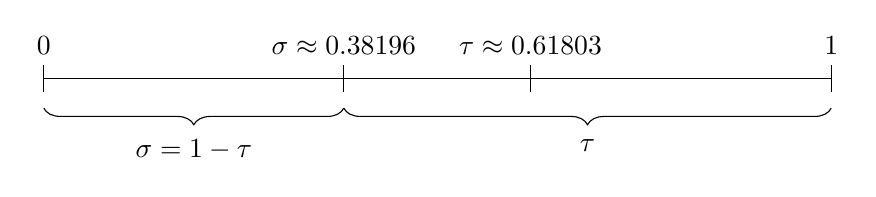
\begin{tikzpicture}
		\draw(0,0)--(10,0);
		\draw(0,-5pt)--(0,5pt) node[above] {$ 0 $};
		\draw(3.81,-5pt)--(3.81,5pt) node[above] {$ \sigma \approx 0.38196 $};
		\draw(6.18,-5pt)--(6.18,5pt) node[above] {$ \tau \approx 0.61803 $};
		\draw(10,-5pt)--(10,5pt) node[above] {$ 1 $};
		\draw[decorate, decoration={brace, mirror, amplitude=6pt}, yshift=-2.5ex] (0,0) -- node[below=1.8ex] {$ \sigma = 1 - \tau $} (3.81,0);
		\draw[decorate, decoration={brace, mirror, amplitude=6pt}, yshift=-2.5ex] (3.81,0) -- node[below=1.8ex] {$ \tau $} (10,0);
	\end{tikzpicture}
}

\newcommand{\plotsigmoid}{%
	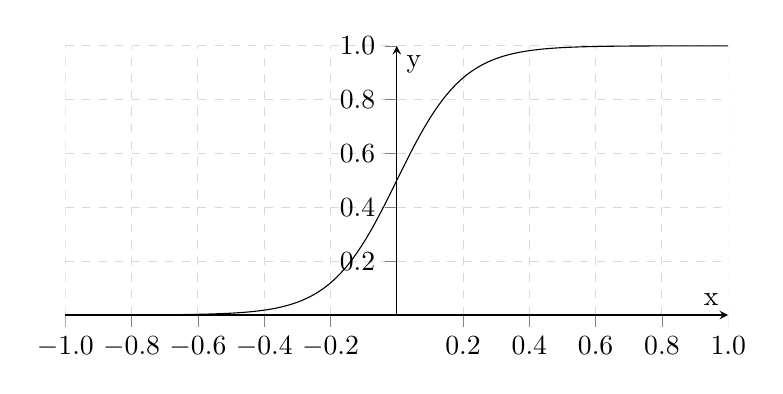
\begin{tikzpicture}
		\begin{axis}[
				legend pos=north west,
				axis x line=middle,
				axis y line=middle,
				x tick label style={/pgf/number format/fixed, /pgf/number format/fixed zerofill,
						/pgf/number format/precision=1},
				y tick label style={/pgf/number format/fixed, /pgf/number format/fixed zerofill,
						/pgf/number format/precision=1},
				grid = major,
				width=10cm,
				height=5cm,
				grid style={dashed, gray!30},
				xmin=-1,
				xmax= 1,
				ymin= 0,
				ymax= 1,
				axis background/.style={fill=white},
				xlabel=x,
				ylabel=y,
				tick align=outside,
				enlargelimits=false]
			\addplot[domain=-1:1,samples=500] {1/(1+exp(-10*x))};
			% \addlegendentry{$ \sigmoid(x) = \frac{1}{1+e^{-x}} $}
		\end{axis}
	\end{tikzpicture}
}

\newcommand{\plotvectorangle}{%
	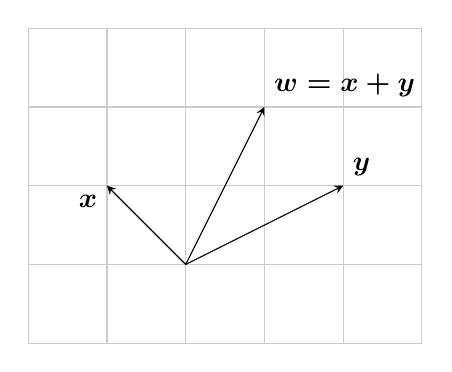
\begin{tikzpicture}
		\draw[thin,gray!40] (-2,-1) grid(3,3);
		\draw[-stealth](0,0) -- (-1,1) node[anchor=north east]{$\boldsymbol{x}$};
		\draw[-stealth](0,0) -- (2,1) node[anchor=south west]{$\boldsymbol{y}$};
		\draw[-stealth](0,0) -- (1,2) node[anchor=south west]{$\boldsymbol{w = x + y}$};
	\end{tikzpicture}
	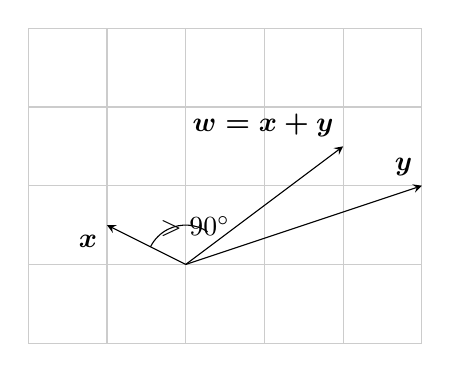
\begin{tikzpicture}
		\draw[thin,gray!40] (-2,-1) grid(3,3);
		\draw[-stealth](0,0) -- (-1,0.5) node[anchor=north east]{$\boldsymbol{x}$};
		\draw[-stealth](0,0) -- (3,1) node[anchor=south east]{$\boldsymbol{y}$};
		\draw[-stealth](0,0) -- (2,1.5) node[anchor=south east]{$\boldsymbol{w = x + y}$};
		\draw [black] (56.30:0.5) arc [start angle=56.30, end angle=153.43, radius=0.5cm]
		node [above right] {$ > \ang{90} $};
	\end{tikzpicture}
}


\newpage
\section{Notes on Analysis}

\begin{lemma}[Some small Calculations]\hfill
    \begin{enumerate}
        \item For \( 1 = x x^{-1} \) the product rule yields \( 0 = x^{-1} + x(x^{-1})' \). Hence
            \[
                \frac{d}{dx} x^{-1} = -\frac{1}{x^2}
            \]
        \item Similarly \( x = \sqrt{x}^2 \) and \( 1 = 2 \sqrt{x} \sqrt{x}' \) and so
            \[
                \frac{d}{dx} \sqrt{x} = \frac{1}{2\sqrt{x}}
            \]
        \item \( (1 - q) (1 + q + q^2 + \ldots + q^n) = 1 - q + q - q^2 + q^2 - q^3 + \ldots + q^{n+1} \) gives
            \[
                \sum_{k=0}^n q^k = \frac{1 - q^{n+1}}{1 - q}
            \]

    \end{enumerate}
\end{lemma}
\bigskip

\begin{theorem}[Fermat Stationary Point]\label{thm:fermat_stationary_point}
Let \( \Omega \subseteq \R \) be open and \( f \in C^1(\Omega) \). If \( x^* \in \Omega \) is local extremum 
then \( f^\prime(x^*) = 0 \).
\end{theorem}

\begin{proof}
Assume \( x^* \) is the minimum of \( f \) in \( \Omega \) and let \( f^\prime(x^*) > 0 \). 
Since \( f \in C^1(\Omega) \) there exist \( \eps, \delta > 0 \), so that for \( |h| \le \eps \)
\[
    \frac{f(x^* + h) - f(x^*)}{h} > \delta
\]
Pick a negative \( h \in [-\eps, 0) \). Then 
\[
     f(x^* + h) < f(x^*) +  \delta h < f(x^*) 
\]
and \( x^* \) cannot be the minimum. Analog for maximum with a positive \( h \), then apply to \( -f \).
\end{proof}
\bigskip


\begin{theorem}[Rolle]\label{thm:rolle}
Let \( f \in C[a,b] \) with \( f(a) = f(b) \). If \( f \) is differentiable in \( (a, b) \) then 
there exists a \( \xi \in (a,b) \) with \( f^\prime(\xi) = 0 \).
\end{theorem}

\begin{proof}
Assume \( f \) is not constant. Since \( [a,b] \) is compact there exists either a global minimum or maximum 
\( \xi \in (a,b) \) and Theorem~\ref{thm:fermat_stationary_point} can be applied.
\end{proof}
\bigskip


\begin{theorem}[Mean Value]\label{thm:mean_value}
Let \( f \in C[a,b] \) be differentiable in \( (a, b) \). Then there exists a \( \xi \in (a,b) \) with 
\[
    f^\prime(\xi) = \frac{f(b) - f(a)}{b - a}
\]
\end{theorem}

\begin{proof}
Apply Theorem~\ref{thm:rolle} to 
\[
    g(x) = f(x) - \frac{f(b) - f(a)}{b - a} (x -a) 
\]
\end{proof}
\bigskip

\begin{remark}\hfill
    \begin{enumerate}
        \item More generally choose any \( \varphi \in C^1[a,b] \) with \( \varphi(a) = 0 \) and 
            \( \varphi(b) = f(b) - f(a) \). Set \( g(x) = f(x) - \varphi(x) \) to see there is a \( \xi \in (a,b) \) 
            with \( f^\prime(\xi) = \varphi^\prime(\xi)\). 
        \item Another useful generalization: let \( \Omega \subseteq \Rn \) be open and \( f \in C^1(\Omega) \). For
            \( x, y \in \Omega \) define \( \varphi(t) = f(tx + (1 - t)y) \) and apply the chain rule for differentiation
            \[
                 \varphi^\prime(\xi) = \gradient {f(\xi x + (1 - \xi)y)}^T(x - y) = f(x) - f(y)
            \]
        \item The Cauchy Schwarz inequality then yields
            \[
                  \|f(x) - f(y)\| \le \|\gradient f(\xi x + (1 - \xi)y)\| \|(x - y)\|
            \]
    \end{enumerate}
\end{remark}
\bigskip

\begin{theorem}[Differentiation Theorem]\label{thm:differentiation}
Let \( f \in C[a,b] \) and define 
\[
    F(x) = \int_a^x f(t)\,dt
\]
Then \( F \in C^1[a,b] \) with \( F^\prime(x) = f(x) \) for \( x \in [a,b] \).
\end{theorem}

\begin{proof}
Applying the Mean Value Theorem of Integration gives
\[
    F(x + h) - F(x) =  \int_x^{x + h} f(t)\,dt = f(\xi) h
\]
for some \( \xi \in (x, x + h) \).
\end{proof}
\bigskip

\begin{theorem}[Fundamental Theorem of Calculus]\label{thm:fund_calculus}
Let \( f \in C[a,b] \). Then
\[
    F(b) -F(a) = \int_a^b f(t)\,dt
\]
\end{theorem}

\begin{lemma}[Directional Derivative]\label{lemma:directional_derivative}
Let \( \Omega \subseteq \Rn \) be open and \( f \in C^1(\Omega) \). Then
\[
    \frac{\partial f}{\partial d}(x) = \gradient{f(x)}^T d
\]
for any \( d \in \Rn \).
\end{lemma}

\begin{proof}
Let \( \varphi(t) = f(x + td) \). Then \( \varphi \in C^1[-\eps, \eps ] \) for some \( \eps > 0 \) 
and the chain rule yields 
\[ 
    \varphi^\prime(t) = {\gradient f(x + td)}^T d 
\]
Hence
\[
    \varphi^\prime(0) = \lim_{t \to 0} \frac{\varphi(x + td) - \varphi(0)}{t} = 
        \lim_{t \to 0} \frac{f(x + td) - f(x)}{t} = {\gradient f(x)}^T d
\]
\end{proof}
\bigskip

\begin{remark}\hfill
    \begin{enumerate}
        \item Note that by definition the directional derivative is invariant under multiplication 
            with any \( \lambda \ne 0 \).

        \item A similar proposition holds under the weaker assumption that \( d \) is a only feasable direction 
            for \( f \) in \( x \)

        \item For \( d = \gradient{f(x)}/\| \gradient{f(x)}\| \) it follows that
            \[
                \frac{\partial f}{\partial d}(x) = \|\gradient{f(x)}\| > 0
            \]
            and for any other \( d \in \Rn \) with \( \|d\| = 1 \) the Cauchy Schwarz inequality yields
            \[
                |\frac{\partial f}{\partial d}(x)| = |\gradient{f(x)}^T d| \le \|\gradient{f(x)}\| \|d\| = 
                    \|\gradient{f(x)}\|
            \]
            Hence \( \gradient{f(x)} \) is the direction of the greatest ascent and respectively, 
            \( -\gradient{f(x)} \) is the direction of the greatest descent.
    \end{enumerate}
\end{remark}
\bigskip

\begin{theorem}[First Order Necessary Condition]\label{thm:fonc}
Let \( \Omega \subseteq \Rn \) be open and \( f \in C^1(\Omega) \). If \( x^* \in \Omega \) is a local minimzer then
\( \gradient f(x^*) = 0 \).
\end{theorem}

\begin{proof}
Let \( h \in \Rn \) and \( \delta > 0 \) so that \( x^* + th \in \Omega \) for all \( t \in (-\delta, \delta) \). 
Then \( 0 \) is local minimizer for \( \varphi(t) = f(x^* + th) \) and
\[
    \varphi^\prime(0) = {\gradient f(x^*)}^T h = 0
\]
Now let \( h = \gradient f(x^*) \). 
\end{proof}
\bigskip


\newpage
\section{Nonlinear Optimization}
\subsection{Minimization without Constraints}
\bigskip


\begin{lemma}[Gradient Inequality]\label{thm:lemma_gradient_inequality}
    Let \(M \subseteq \mathbb{R}^n \) be a convex set and \(f \in C^1(M)\). Then \(f\) is convex if and only if
    \[
        f(x) \ge f(y) + \gradient {f(y)}^T (x - y)
    \]
    for all \(x, y \in M \).
\end{lemma}

\begin{proof}
    Let f be convex and \(x, y \in M\). For \( 0 \le \lambda \le 1 \) follows
    \[
        f(\lambda x + (1 - \lambda) y) \le \lambda f(x) + (1 - \lambda)f(y) =  \lambda f(x) - \lambda f(y) + f(y)
    \]
    and
    \[
        f(x) - f(y) \ge \frac{f(\lambda x + (1 - \lambda) y) - f(y)}{\lambda}
        = \frac{f(y + \lambda (x - y)) - f(y)}{\lambda}
    \]
    For \( d = x - y \)\ and \( \lambda \to 0 \) the term on the right converges to the direction derivative of \( f \)
    in \( d \)
    \[
        \frac{\partial f}{\partial d}(y) = \gradient{f(y)}^T d = \gradient{f(y)}^T (x - y)
    \]

    Now let \( x, y \in M \) and  \( 0 \le \lambda \le 1 \). For \( z = \lambda x + (1 - \lambda) y \in M \)
    it follows that
    \[
        \begin{split}
            \lambda f(x) & \ge \lambda f(z) + \lambda \gradient {f(z)}^T (x - z) \\
            (1 - \lambda) f(y) & \ge (1 - \lambda) f(z) + (1 - \lambda) \gradient {f(z)}^T (y - z)
        \end{split}
    \]
    Adding the two inequalities gives
    \[
        \begin{split}
            \lambda f(x) + (1 - \lambda) f(y)
            & \ge f(z) + \gradient {f(z)}^T(\lambda x - \lambda z + (1- \lambda) y - (1-\lambda)z) \\
            & = f(z) + \gradient {f(z)}^T(\lambda x + (1- \lambda) y - z) \\
            & = f(z)
        \end{split}
    \]
\end{proof}
\bigskip


\begin{exercise}[Facility Locations]
    The facilities are located at:
    \[
        (3, 0), (0, -3), (1, 4)
    \]
\end{exercise}

\begin{proof}
    Let
    \[
        \begin{split}
            f(x)    & = {(x - 3)}^2 + y^2 + x^2 + {(y + 3)}^2 + {(x - 1)}^2 + {(y - 4)}^2 \\
            & = x^2 - 6x + 9 + y^2 + x^2 + y^2 + 6y + 9 + x^2 - 2x + 1 + y^2 -8y + 16 \\
            & = 3x^2 + 3y^2 - 8x - 2y + 35
        \end{split}
    \]
    Then
    \[
        \gradient f(x, y) = (6x - 8, 6y - 2) \text{ and } \gradient^2 f(x, y) =
        \begin{pmatrix}
            6 & 0 \\
            0 & 6 \\
        \end{pmatrix} > 0
    \]
    Hence \( (4 / 3, 1 / 3) \) is the gobal minimum.
\end{proof}
\bigskip


\exercise[Convex Functions]
The sum of convex functions is convex.

\proof{}
Let \( x, y \in M \). Since \( \alpha_i  > 0 \) it is
\[
    \begin{split}
        f(\lambda x + (1 - \lambda) y)
        & = \sum_{i=1}^m \alpha_i f_i(\lambda x + (1 - \lambda) y) \\
        & \le \sum_{i=1}^m \alpha_i \lambda f_i(x) + \sum_{i=1}^m \alpha_i (1 - \lambda) f_i(y)
        =  \lambda f(x) + (1 - \lambda) f(y)
    \end{split}
\]
Let \( f(x) = x^2 \). Then \( -f \) is not convex, e.g. \( x = 1, y = -1 \) and \( \lambda = 0.5 \).
\bigskip


\exercise[Solution of Quadratic Inequality]
Let
\[
    f(x) = x^{T}Ax + b^{T}x + c
\]
\proof{}
The product rule gives
\[
    \gradient {f(x)} = x^{T}A + Ax + b = (A^{T} + A)x + b = 2Ax + b
\]
Thus \( \hessian {f(x)} = 2A > 0 \) and \( f \) is convex. Hence the level set \( \Gamma_{-c} \) is convex.
Since the intersection of convex sets is convex \( \Gamma_{-c} \cap \{ x \in \Rn: g^{T}x + h = 0 \} \)
is convex, too.
\bigskip


\exercise[Line Search on Compact Convex Sets]
Let \( S \subset \mathbb{R}^n \) be compact and convex. Furthermore let \( f \in C^1(S) \) be convex,
\( x \in S \) and \( d \in \mathbb{R}^n \) a descent direction of \( f \) in \( x \)
with \( \gradient {f(x)}^T d < 0 \).

\proof{}
If  \( x + \lambda^* d \) is an optimal solution then \( \gradient {f(x + \lambda^* d)}^T d = 0 \)
according to Theorem~\ref{thm:fonc}.
Let \( \gradient {f(x + \lambda^* d)}^T d = 0 \). Then Lemma~\ref{thm:lemma_gradient_inequality} gives
\[
    f(x + \lambda d) \ge f(x + \lambda^* d) + (\lambda - \lambda^*) \gradient {f(x + \lambda^* d)}^T d
    = f(x + \lambda^* d)
\]
and \( x + \lambda^* d \) is an optimal solution.
\bigskip


\begin{exercise}[Steepest Descent]
    Let
    \[
        f(x) = \frac{1}{2} x^T{A}x + b^T x + c
    \]
    where \( A \) is symmetrical and positive definite.
\end{exercise}

\begin{proof}
    Since \( \gradient {f(x)} = Ax + b \) and \( \hessian {f(x)} = A > 0 \) it follows \( x^* = -A^{-1}b \).
    Let \( v \) be eigenvector with \( Av = \mu v \). For \( x_0 = x^* + \theta v \) it follows
    \[
        \gradient {f(x_0)} = Ax^* + \mu \theta v + b = \mu \theta v
    \]
    and for \(\lambda \ge 0 \)
    \[
        \argmin \{ f(x_0 - \lambda \gradient f(x_0)) \} =
        \argmin \{ f(x^* + \theta v - \lambda \mu \theta v)\} = \mu^{-1}
    \]
    Thus
    \[
        x_1 = x_0 - \mu^{-1} \gradient f(x_0) = x^* + \theta v - \mu^{-1} \mu \theta v = x^*
    \]
    and \( \gradient {f(x_1)} = 0 \). Hence the algorithm stops after the first iteration.
    Now let
    \[
        x_0 = x^* + \sum_{i=0}^m \theta_i v_i
    \]
    for orthogonal eigenvectors with \( Av_i = \mu_i\) and \( m \le n \). Then
    \[
        \gradient {f(x_0)} = Ax^* + \sum_{i=0}^m \mu_i \theta_i v_i + b = \sum_{i=0}^m \mu_i \theta_i v_i
    \]
    and
    \[
        x_1 = x_0 - \lambda \sum_{i=0}^m \mu_i \theta_i v_i
        = x^* + \sum_{i=0}^m \theta_i v_i - \lambda \sum_{i=0}^m \mu_i \theta_i v_i
        = x^* + \sum_{i=0}^m (1 - \lambda \mu_i) \theta_i v_i
    \]
    Since \( x^* \) is the minimum it follows \( \gradient {f(x_1)} = 0 \) iff \( \lambda = \mu^{-1} \)
    for all \( 0 \le i \le m \).
\end{proof}
\bigskip



\subsection{One Dimensional Minimization and Direct Search}
\bigskip


\begin{definition}[Unimodal Function]\label{def:unimodal_fnc}
    A function \( f : [a,b] \to \R \) is called unimodal if there exists a \( \xi \in [a,b] \), so that
    \( f \) is strictly decreasing in \( [a, \xi] \) and strictly increasing in \( [\xi, b] \).
\end{definition}
\bigskip

In fact \( \xi \) is the unique minimum of \( f \) in \( [a, b] \). According to the definition,
for \( a \le x < y \le b \) follows
\[
    f(x) > f(y) \text{ for } x, y \in [a, \xi) \text{ and } f(x) < f(y) \text{ for }  x, y \in (\xi, b]   % chktex 9
\]
Thus
\[
    \xi \in [a, y] \text{ if } f(x) < f(y) \text{ and } \xi \in [x, b] \text{ if } f(x) \ge f(y)
\]

Consider now a symmetrical partioning of the interval \( [0, 1] \) where two consecutive partionings hold
the same ratio respectively:
\[
    \sigma = 1 - \tau \text{ and } \frac{1}{\tau} = \frac{\tau}{\sigma}
\]
Then \( 1 - \tau = \tau^2 \) and solving the quadratic equation \( \tau^2 + \tau = 1 \) yields
\[
    \tau = \frac{\sqrt{5} - 1}{2} \approx 0.61803
\]
\bigskip

\begin{figure}[H]
    \centering
    \plotgoldensection{}
    \caption{Golden Section}\label{fig:golden_section}
\end{figure}
\bigskip

Let now \( [a_0, b_0] = [a, b] \) and define
\[
    [a_{k + 1}, b_{k + 1}] =
    \begin{cases}
        [a_k, y_k] & \text{ if } f(x_k) < f(y_k)   \\
        [x_k, b_k] & \text{ if } f(x_k) \ge f(y_k)
    \end{cases}
\]
where
\[
    \begin{split}
        x_k & = b_k - \tau (b_k - a_k) \\
        y_k & = a_k + \tau (b_k - a_k)
    \end{split}
\]
It follows that \( [a_k, b_k] \supset [a_{k + 1}, b_{k + 1}] \) is a decreasing series of intervals with
\[
    (b_{k + 1} - a_{k + 1}) =  \tau(b_k - a_k)
\]
where the interval converges to \( \xi \). This leads to the following algorithm:
\bigskip

\begin{algorithm}[Golden Section Search]\label{algo:golden_section_search}
\end{algorithm}
\inputminted[fontsize=\small, framesep=0.35cm, frame=lines, python3=true]{python}{../jupyter/calculus/golden_section.py}
\bigskip

\begin{exercise}[Surprising Convergence]
    Example for \( f \in C^2(\mathbb{R}) \) with a sequence of strict local minima converging to a strict local maximum.
\end{exercise}
\bigskip


\subsection{Methods of Steepest Descent}
\bigskip


\begin{definition}
    Let \( f \in C^1(\Rn) \) and \( x_0 \in \Rn \) an arbitraty starting point.
    \begin{enumerate}
        \item For sequences \( \lambda_k > 0 \) and unit vectors \( s_k \in \Rn \) define
              \[
                  x_{k + 1} = x_k + \lambda_k s_k
              \]
        \item Assume there exists \( 0 < \alpha \le 1 \) so that
              \[
                  - \gradient f(x_k) s_k \ge \alpha \|\gradient f(x_k)\|
              \]
        \item Furthermore assume that for some \( 0 < \beta \le \gamma < 1 \) the following inequalities hold
              \[
                  f(x_{k + 1}) \le f(x_k) + \lambda_k \beta \gradient f(x_k) s_k
              \]
              \[
                  \gradient f(x_{k + 1}) s_k \ge \gamma \gradient f(x_k) s_k
              \]
    \end{enumerate}
    Then \( \lambda_k \) and  \( s_k \) are called \emph{step lengths} and \emph{search directions} respectively
    and \( x_k \) is called a \emph{sequence of descent} for \( f \).
\end{definition}
\bigskip


\begin{remarks}
    The inequalities above serve different purposes
    \begin{enumerate}
        \item  It is
              \[
                  - \gradient f(x_k) s_k = \cos\varphi \|\gradient f(x_k)\| \|s_k\| =
                  \cos\varphi \|\gradient f(x_k)\| \ge \alpha \|\gradient f(x_k)\|
              \]
              Hence the angle between the direction of the steepest descent and the search direction is
              strictly smaller then \( \ang{90} \) degrees.
        \item  Since \( \gradient f(x_k) s_k \le 0 \) it follows
              \[
                  f(x_{k + 1}) \le f(x_k) + \beta \lambda_k \gradient f(x_k) s_k \le f(x_k)
              \]
              and \( f(x_k) \) is monotonically decreasing.
        \item Furthermore
              \[
                  \gradient f(x_{k + 1}) s_k = \gradient f(x_k + \lambda_k s_k) s_k
                  \ge \gamma \gradient f(x_k) s_k
              \]
              Hence the step length cannot be chosen too small due to the continuity of the dervative.
    \end{enumerate}
\end{remarks}
\bigskip


% \begin{theorem}[Steepest Descent Method]\label{thm:steepest_descent}
%     Let \( f \in C^2(\Rn) \) and \( x_k \) a sequence of descent for \( f \).
%     Then every accumulation point of \( x_k \) is a stationary point of \( f \).
% \end{theorem}

% \begin{proof}
% \end{proof}

\newpage
\section{Functional Analysis}

\subsection{The Hahn-Banach Theorem}
\bigskip

\begin{remarks}
    \hfill
    \begin{enumerate}
        \item Let \( f = u + \iu v\) be a complex valued linear functional.
              Then \( f(\iu x) = \iu f(x) \) gives
              \[
                  u(\iu x) = -v(x) \text{ and } v(\iu x) = \iu u(x)
              \]
              Thus
              \[
                  f(x) = u(x) - \iu u(\iu x)
              \]
        \item Assume \( |u(x)| \le C\|x\| \) and choose \( t \in \R \) so that \( |f(x)| = e^{\iu t}f(x) \).
              Then
              \[
                  |f(x)| = e^{\iu t}f(x) = f(e^{\iu t}x) = u(e^{\iu t}x) \le C\|e^{\iu t}x\| = C\|x\|
              \]
        \item
              See also the \hyperref[thm:thm_cauchy_riemann_eqations]{Cauchy-Rieman 
              Eqautions~\ref*{thm:thm_cauchy_riemann_eqations}}.
    \end{enumerate}
\end{remarks}
\bigskip


\begin{theorem}[Hahn-Banach Theorem]\label{thm:hahn_banach}
    Let \( E \) be a normed space and \( F \) a linear subspace. For any linear functional
    \( f \in F^* \) there exists a \( \tilde{f} \in E^* \) so that
    \[
        \tilde{f}|_F = f \text{ and } \|\tilde{f}\| = \|f\|
    \]
\end{theorem}

\begin{proof}
    Assume that \( f: E \to \R \) is a real valued linear functional and \( x' \in E \setminus F \).
    Consider the subspace \( F' = \{x + \lambda x' | x \in F \} \) and define
    \[
        f'(x + \lambda x') = f(x) + \lambda r
    \]
    for some \( r \in \R \).  As sum of two linear functionals \( f' \) again is a linear functional with
    \( \|f'\| \ge \|f\| \).

    Determine \( \lambda \), so that the inequality holds.

    Using Zorn's Lemma allows the extension to \( E \) while the remarks above can be used to extend
    to complex valued linear functionals.
\end{proof}
\bigskip


\subsection{The Riesz Representation Theorem}
\bigskip

\begin{theorem}[The Riesz Representation Theorem]\label{thm:riesz_representation}
    Let \( X \) be a locally compact Hausdorff space and \( L \in C_c(X) \) a positive linear functional. 
    Then ther exists a \( \sigma \)-algebra \( M \) in \( X \) and a unique positive measure 
    \( \mu \) on \( M \) so that
    \[
        L(f) = \int_X f\,d\mu
    \]
    for every \( f \in C_c(X) \).
\end{theorem}
\bigskip


\newpage
\section{Neural Networks}

\subsection{The Perceptron}

\begin{definition}[Binary Classifiers]
	Let \( X \subset \R^n \) be the union of two disjoint finite sets \( X = M \cup N \).
    \begin{enumerate}
		\item A \emph{binary classification problem} is the task to find a mapping \( f: X \to \{ 0, 1 \} \) with
			\[
				% f(x) = 1 \text{ for } x \in M \text{ and } f(x) = 0 \text{ for } x \in N
		        f(x) = \left\{
		            \begin{array}{ll}
		                1& \text{for } x \in M \\
		                0& \text{for } x \in N
		            \end{array}
			\]
			\( f \) then is called a \emph{binary classifier} for \( X \)
		\item \( X \) is called \emph{separable} if there exists a \emph{weight vector} \( w \in \R^n \) 
			and a \emph{bias} \( b \in \R \) so that
				\[
					\begin{split}
						wx + b & > 0 \text{ for } x \in M \\
						wx + b & < 0 \text{ for } x \in N
					\end{split}
				\]
		\item The weight \( w \) and the bias \( b \) are called \emph{solution to the classification problem}. 
		    They implicitely define a binary classifier via
				\[
		        f(x) = \left\{
		            \begin{array}{ll}
		                1& \text{ if } wx + b > 0 \\
		                0& \text{ if } wx + b < 0
		            \end{array}
				\]
    \end{enumerate}
\end{definition}
\bigskip


\begin{examples}\hfill
    \begin{enumerate}
        \item Let \( X = \{ 0, 1 \} \times \{ 0, 1 \} \) and consider the \emph{and} operator 
		    \( f(1, 1) = 1 \) and \( f(x, y) = 0 \) elsewhere. Then \( w = (3, 3) \) and \( b = -5 \) 
			yield a solution to the classification problem \( M = f^{-1}(1) \) and \( N = f^{-1}(0) \)
        \item Again let \( X = \{ 0, 1 \} \times \{ 0, 1 \} \) and \( f(1, 0) = f(0, 1) = 1 \) and 
			\( f(0, 0) = f(1, 1) = 0 \), the \emph{xor} operator. Thus for any weight \( (w_1, w_2) \) and 
			any bias \( b \)
				\[
					\begin{split}
						w_1 + b & > 0 \\ 
						w_2 + b & > 0 \\
						\\
						w_1 + w_2 + b & \le 0 \\
					    b & \le 0
					\end{split}
				\]
			Adding two equations respectively shows that there is no solution
		\item The bias can be integrated into the weight vector via \( w' = (w, b) \in \R^{n + 1} \) and 
			\( x' = (x, 1) \in \R^{n + 1} \). Separability then reduces to
				\[
					w'x' > 0
				\]
	\end{enumerate}
\end{examples}
\bigskip


\subsubsection*{Geometrical Interpretation}
The idea for the perceptron most likely has its origin in a simple geometrical observation.
Recall that for \( x, y \in \R^n \) the dot product can be expressed as 
\[
	xy = \|x\| \|y\| \cos \alpha 
\]
where \( \alpha \) is the angle between the two vectors. Hence the product is positive 
if the angle is less than \( \ang{90} \) degrees and negative if the angle is between \( \ang{90} \) 
and \( \ang{180} \) degrees
\[
	xy > 0 \text{ for } 0 \le \alpha < \pi / 2 \text{ and } xy < 0 \text{ for } \pi / 2 < \alpha \le \pi
\]
Note, that the sign does not dependend on lengths of the vectors, but solely on the angle.

For any two vectors it is easy enough to find a weight that satisfies \( wx > 0 \) and \( wy > 0 \). 
Generally \( w = x + y \) is a good guess, but not always correct as shown below in 
\hyperref[fig:vectorangle]{Figure \ref*{fig:vectorangle}}. 

\bigskip
\begin{figure}[H]
	\centering
	\plotvectorangle
	\caption{Dot Product and Angle}\label{fig:vectorangle}
\end{figure}
\bigskip

But, the more similar the lengths of the two vectors are the more likely \( x + y \) works. 
Actually the threshold is tbd.
An iterative approach is to increase \( w = x + y \) in the direction of vector with the angle greater 
than \( \ang{90} \) degrees.

\begin{examples}\hfill
    \begin{enumerate}
        \item Let \( x = (-1, 1) \) and \( y = (6, 1) \). Then 
			\[ 
				\begin{align*}
					w_0 &= (5, 2) & w_0x &= -3 < 0 & w_0y &= 32 > 0 \\
					w_1 &= (4, 3) & w_1x &= -1 < 0 & w_1y &= 27 > 0 \\
					w_2 &= (3, 4) & w_2x &= 1 > 0 & w_2y &= 22 > 0 \\
				\end{align*}
			\]
        \item Let \( x = (4, -6) \) and \( y = (-10, 5) \). Then 
			\[ 
				\begin{align*}
					w_0 &= (-6, -1) & w_0x &= -18 < 0 & w_0y &= 55 > 0 \\
					w_1 &= (-2, -7) & w_1x &= 34 > 0 & w_1y &= -15 < 0 \\
					w_2 &= (-12, -2) & w_2x &= -36 < 0 & w_2y &= 110 > 0 \\
					w_3 &= (-8, -8) & w_3x &= 16 > 0 & w_3y &= 40 > 0 \\
   				\end{align*}
			\]
    \end{enumerate}
\end{examples}
	

\begin{algorithm}[Weight]\label{algo:weight}
\end{algorithm}
\inputminted[fontsize=\small, framesep=0.35cm, frame=lines, python3=true]{python}{python/weight.py}
\bigskip



\begin{algorithm}[Perceptron]\label{algo:perceptron}
\end{algorithm}
\inputminted[fontsize=\small, framesep=0.35cm, frame=lines, python3=true]{python}{python/perceptron.py}
\bigskip


\subsection{The Backtracking Algorithm}

\begin{definition}[Activation Functions]\hfill
    \begin{enumerate}
		\item The \emph{Heaviside} function \( H: \R \to \{ 0, 1 \} \) is defined as
			\[
				H(x) = \left\{
					\begin{array}{ll}
						1 & \text{ for } x > 0 \\
						0 & \text{ for }x \le 0
					\end{array} 
				\right.
			\]
		\item The \emph{sigmoid} function \( \sigmoid \in C^\infty(\R) \) is defined as 
			\[
				\sigmoid(x) = \frac{1}{1 + e^{-x}}
			\]
    \end{enumerate}
\end{definition}
\bigskip


\begin{figure}[H]
	\centering
	\plotsigmoid
	\caption{The sigmoid function $ \sigmoid(x) = \frac{1}{1 + e^{-x}} $}\label{fig:sigmoid}
\end{figure}
\bigskip


\begin{remarks}\hfill
    \begin{enumerate}
		\item Since the heaviside function is not continous and therefore not differentiable at \( 0 \)
			the sigmoid function is often considered its smooth counterpart
		\item The definition of the sigmoid function yields \( 0 < \sigmoid(x) <  1 \) as well as 
			\( \sigmoid(x) \to 0 \) for \( x \to -\infty \) and \( \sigmoid(x) \to 1 \) for \( x \to \infty \)
		\item The quotient rule yields
			\[
				\sigmoid'(x) 
					= -\frac{-e^{-x}}{(1 + e^{-x})^2}
					= \sigmoid(x) \frac{1 + e^{-x} - 1}{1 + e^{-x}}
					= \sigmoid(x)(1 - \sigmoid(x))
			\]
			and \( \sigmoid \) is monotonically increasing over its domain
    \end{enumerate}
\end{remarks}
\bigskip



\newpage
\section{Neural Networks}

\subsection{The Perceptron}

\begin{definition}[Binary Classifiers]
    Let \( X \subset \R^n \) be the union of two finite disjoint sets \( X = M \cup N \).
    \begin{enumerate}
        \item A \emph{binary classification problem} is the task to find a mapping \( f: X \to \{ 0, 1 \} \) with
              \[
                  f(x) = \left \{
                  \begin{array}{ll}
                      1 & \text{ for } x \in M \\
                      0 & \text{ for } x \in N
                  \end{array}
                  \right.
              \]
              \( f \) then is called a \emph{binary classifier} for \( X \)
        \item \( X \) is called \emph{separable} if there exists a \emph{weight vector} \( w \in \R^n \)
              and a \emph{bias} \( b \in \R \) so that
              \[
                  \begin{split}
                      wx + b & > 0 \hspace{1em}\text{ for } x \in M \\
                      wx + b & < 0 \hspace{1em}\text{ for } x \in N
                  \end{split}
              \]
        \item The weight \( w \) and the bias \( b \) are called \emph{solution to the classification problem}.
              They implicitly define a binary classifier via
              \[
                  f(x) = \left \{
                  \begin{array}{ll}
                      1 & \text{ if } wx + b > 0 \\
                      0 & \text{ if } wx + b < 0
                  \end{array}
                  \right.
              \]
    \end{enumerate}
\end{definition}
\bigskip


\begin{examples}
    \hfill
    \begin{enumerate}
        \item Let \( X = \{ 0, 1 \} \times \{ 0, 1 \} \) and consider the \emph{and} operator
              \( f(1, 1) = 1 \) and \( f(x, y) = 0 \) elsewhere. Then \( w = (3, 3) \) and \( b = -5 \)
              yield a solution to the classification problem \( M = f^{-1}(1) \) and \( N = f^{-1}(0) \)
        \item Again let \( X = \{ 0, 1 \} \times \{ 0, 1 \} \) and \( f(1, 0) = f(0, 1) = 1 \) and
              \( f(0, 0) = f(1, 1) = 0 \), the \emph{xor} operator. Thus for any weight \( (w_1, w_2) \) and
              any bias \( b \)
              \[
                  \begin{split}
                      w_1 + b & > 0 \\
                      w_2 + b & > 0 \\
                      \\
                      w_1 + w_2 + b & \le 0 \\
                      b & \le 0
                  \end{split}
              \]
              Adding two equations respectively shows that there cannot be a solution
        \item The bias can be integrated into the weight vector via \( w' = (w, b) \in \R^{n + 1} \) and
              \( x' = (x, 1) \in \R^{n + 1} \). Separability then reduces to
              \[
                  w'x' > 0
              \]
    \end{enumerate}
\end{examples}
\bigskip


\subsubsection*{Geometrical Interpretation}
The idea for the perceptron most likely has its origin in a simple geometrical observation.
Recall that for \( x, y \in \R^n \) the dot product can be expressed as
\[
    xy = \|x\| \|y\| \cos\alpha
\]
where \( \alpha \) is the angle between the two vectors. Hence the product is positive
if the angle is less than \( \ang{90} \) degrees and negative if the angle is between \( \ang{90} \)
and \( \ang{180} \) degrees
\[
    \begin{split}
        xy & > 0 \hspace{1em}\text{ for } 0 \le \alpha < \pi / 2 \\
        xy & < 0 \hspace{1em}\text{ for } \pi / 2 < \alpha \le \pi
    \end{split}
\]
Note, that the sign does not depend on the vector lengths, but solely on the angle.

For any two vectors it is easy enough to find a weight that satisfies \( wx > 0 \) and \( wy > 0 \).
Generally \( w = x + y \) is a good guess, but not always correct as shown below in
\hyperref[fig:vectorangle]{Figure~\ref*{fig:vectorangle}}.

\bigskip
\begin{figure}[H]
    \centering
    \plotvectorangle{}
    \caption{Dot Product and Angle}\label{fig:vectorangle}
\end{figure}
\bigskip

But, the more similar the lengths of the two vectors are the more likely \( x + y \) works.
The actual threshold is given by the following
\bigskip

\begin{lemma}
    Let \( x, y \in \Rn \) with \( \|x\| < \|y\| \) and \( xy = \|x\| \|y\| \cos\alpha \). If
    \[
        \|x\| > -\|y\|\cos\alpha
    \]
    then \( x(x + y) > 0 \).
\end{lemma}

\begin{proof}
    Let \( x(x + y) = \|x\| \|x + y\| \cos\beta \). Since
    \[
        x(x + y) = xx + xy = {\|x\|}^2 + \|x\| \|y\| \cos\alpha
    \]
    it follows
    \[
        {\|x + y\|}\cos\beta = \|x\| + \|y\|\cos\alpha
    \]
    Hence \( \cos\beta > 0 \) if the inequality above holds.
\end{proof}
\bigskip


An iterative approach is to repeatedly increase \( w = x + y \) in the direction of the shorter vector 
aka the one with the angle greater than \( \ang{90} \) degrees.
\[
    w' = \left \{
    \begin{array}{ll}
        w + x & \text{ if } w x \le 0 \\
        w + y & \text{ if } w y \le 0 \\
    \end{array}
    \right.
\]

While this seems reasonable it is unclear whether the algorithm always yields a result after 
a finite number of iterations. The answer to this question will be given later as a special case 
of the \hyperref[thm:perceptron_convergence]{Perceptron Convergence Theorem~\ref*{thm:perceptron_convergence}}
\bigskip


\begin{algorithm}[Weight]\label{algo:weight}
\end{algorithm}
\inputminted[fontsize=\small, framesep=0.35cm, frame=lines, python3=true]{python}{python/weight.py}
\bigskip


\begin{examples}
    \hfill
    \begin{enumerate}
        \item Let \( x = (-1, 1) \) and \( y = (6, 1) \). Then
              \[
                  \begin{aligned}
                      w_0 & = (5, 2) & w_0x & = -3 & w_0y & = 32 \\
                      w_1 & = (4, 3) & w_1x & = -1 & w_1y & = 27 \\
                      w_2 & = (3, 4) & w_2x & = 1  & w_2y & = 22 \\
                  \end{aligned}
              \]
        \item Let \( x = (4, -6) \) and \( y = (-10, 5) \). Then
              \[
                  \begin{aligned}
                      w_0 & = (-6, -1)  & w_0x & = -18 & w_0y & = 55  \\
                      w_1 & = (-2, -7)  & w_1x & = 34  & w_1y & = -15 \\
                      w_2 & = (-12, -2) & w_2x & = -36 & w_2y & = 110 \\
                      w_3 & = (-8, -8)  & w_3x & = 16  & w_3y & = 40  \\
                  \end{aligned}
              \]
        \item
              Let \( w = x / \|x\| + y/ \|y\| \). Then
              \[
                  wx = \frac{{\|x\|}^2}{\|x\|} + \frac{yx}{\|y\|} = \|x\| + \|x\|\cos\alpha = (1 + \cos\alpha)\|x\| > 0
              \]
              and on the other hand \( wx = \|w\| \|x\| \cos\beta \). Similarily
              \( wy = (1 + \cos\alpha)\|y\| = \|w\| \|y\| \cos\gamma \). Hence
              \[
                  1 + \cos\alpha = \|w\|\cos\beta = \|w\|\cos\gamma
              \]
              and thus \( \beta = \gamma \). Also, as expected, \( wx > 0 \) and \( wy > 0 \)
        \item Task: for any given integer \( k \) find two vectors so that more than \( k \) steps are needed
    \end{enumerate}
\end{examples}
\bigskip


The following theorem is the generalization of the approach above for binary classifiers. 
Roughly sepaking the algorithm changes the weight only for misqualified vectors. The proof measures 
the change of angle against the change of length of the weight vector and provides an estimation 
for the maximumn number of required steps.
\bigskip

\begin{theorem}[Perceptron Convergence Theorem]\label{thm:perceptron_convergence}
    Let \( X = M \cup N \) be separable by \( w^*\in \Rn \). Define \( w_0 = 0 \)
    and repeat to iterate over all \( x \in X \) via
    \[
        w_{k + 1} = \left \{
        \begin{array}{ll}
            w_k + x & \text{ if } x \in M \text{ and } w_k x \le 0 \\
            w_k - x & \text{ if } x \in N \text{ and } w_k x \ge 0 \\
            w_k     & \text{ else }                                \\
        \end{array}
        \right.
    \]
    until no further changes occurr. Suppose \( \|x\| \le r \)  and \( w^*x \ge \delta > 0 \) 
    for \( x \in X \). Then the number of iterations before the algorithm stops is limited by
    \[
        k\le \frac{r^2}{\delta^2}
    \]
\end{theorem}

\begin{proof}
    Let \( x \in M \) with \( w_k x \le 0 \). Then
    \[
        w^*w_{k + 1} = w^*w_k + w^*x \ge w^*w_k + \delta
    \]
    Furthermore
    \[
        \|w_{k + 1}\|^2 = \|w_k + x\|^2 = \|w_k\|^2 + 2w_k x + \|x\|^2 \le \|w_k\|^2 + r^2
    \]

    The same estimations hold for \( x \in N \) with \( w_k x \ge 0 \) and using induction yields
    \[
        w^*w_k \ge k\delta \text{ and } \|w_k\|^2 \le kr^2
    \]
    Assuming \( \|w^*\| = 1\) now gives
    \[
        k^2\delta^2 \le \|w_k\|^2 \le kr^2
    \]
    which proves the initial inequality.
\end{proof}
\bigskip


\begin{algorithm}[Perceptron]\label{algo:perceptron}
\end{algorithm}
\inputminted[fontsize=\small, framesep=0.35cm, frame=lines, python3=true]{python}{python/perceptron.py}
\bigskip


\begin{remark}
    Check \hyperref[thm:banach_fix_point]{Banach Fixed-Point Theorem~\ref*{thm:banach_fix_point}} 
    for an alternative proof?!
\end{remark}
\bigskip


\subsection{Feedforward Neural Networks}

\begin{definition}[Activation Functions]
    \hfill
    \begin{enumerate}
        \item The \emph{Heaviside} function \( H: \R \to \{ 0, 1 \} \) is defined as
              \[
                  H(x) = \left \{
                  \begin{array}{ll}
                      1 & \text{ for } x > 0  \\
                      0 & \text{ for }x \le 0
                  \end{array}
                  \right.
              \]
        \item The \emph{sigmoid} function \( \sigmoid \in C^\infty(\R) \) is defined as
              \[
                  \sigmoid(x) = \frac{1}{1 + e^{-x}}
              \]
        \item A function \( s: \R \to \R \) with \( s(x) \to 0 \) 
              for \( x \to -\infty \) and \( s(x) \to 1 \) for \( x \to \infty \) is called a 
              \emph{sigmoidal activation function}
      \end{enumerate}
\end{definition}
\bigskip


\begin{remarks}
    \hfill
    \begin{enumerate}
        \item Since the heaviside function is not continuous and therefore not differentiable 
            at \( 0 \) the sigmoid function can be considered its smooth counterpart
        \item The definition of the sigmoid function yields \( 0 < \sigmoid(x) < 1 \) as well as
              \( \sigmoid(x) \to 0 \) for \( x \to -\infty \) and \( \sigmoid(x) \to 1 \) 
              for \( x \to \infty \)
        \item The quotient rule yields
              \[
                  \sigmoid'(x)
                  = -\frac{-e^{-x}}{{(1 + e^{-x})}^2}
                  = \sigmoid(x) \frac{1 + e^{-x} - 1}{1 + e^{-x}}
                  = \sigmoid(x)(1 - \sigmoid(x))
              \]
              and \( \sigmoid \) is monotonically increasing over its domain
    \end{enumerate}
\end{remarks}
\bigskip


\begin{figure}[H]
    \centering
    \plotsigmoid{}
    \caption{The sigmoid function \( \sigmoid(x) = \frac{1}{1 + e^{-x}} \)}\label{fig:sigmoid}
\end{figure}
\bigskip


\begin{definition}[Single Layer Neural Network]
    Let \( w_k \in \R^n \) and \( b_k \in \R \). For \( \alpha_k \in \R \) define \( f : \Rn \to \R \)
    \[
        f(x) = \sum_{k = 0}^m \alpha_k \sigmoid(w_k x + b_k)
    \]
    The \( f \) is called a \emph{feedforward neural network} of \( m \) units.
\end{definition}
\bigskip

\begin{theorem}[The Universal Approximation Theorem]\label{thm:universal_approximation}
    The subspace of all single layer feedforward neural networks is dense in \( C(I^n) \).
\end{theorem}


\begin{remarks}
    \hfill
    \begin{enumerate}
        \item Let \( f = (f_1, f_2, \dots f_n) : \Rn \to \Rm \) and 
            \[ 
                g(x) = \|f(x)\|^2 = \sum_{j = 1}^m {f_j(x)}^2 
            \] 
        Then
            \[ 
                \frac{\partial g_j}{\partial x_i}(x)
                    = \sum_{j = 1}^m \frac{\partial f_j^2}{\partial x_i}(x)
                    = 2 \sum_{j = 1}^m \frac{\partial f_j}{\partial x_i}(x) f_j(x)
            \] 
        Hence
        \[ 
            \gradient g(x) = 2 \sum_{j = 1}^m \gradient f_j(x) f_j(x)
        \] 

    \end{enumerate}
\end{remarks}
\bigskip


\begin{definition}[Error Function]
    Let \( w \in \R^{n \times m} \) and \( b \in \Rm \). For a finite \emph{test set} \( T \subset \Rn \times \Rm \) 
    define the \emph{error function}
    \[
        E(w,b) = \sum_{(x,y) \in T} \|\sigmoid(wx + b )- y\|^2
    \]
\end{definition}
\bigskip

\subsection{The Backpropagation Algorithm}

\end{document} 
